% ---------------------------------------------------------------------------
% BODY of the paper, \input by the wrapper main.tex (ACM sigconf, WWW 2027;
% the Overleaf main document). Edit the text HERE; the wrapper carries only the
% preamble, title, abstract and bibliography. Keep it format-neutral: no
% \usepackage, no \bibliography.
%
% 2026-10-20: restructured (user): intro with a contribution list / related /
% benchmark (task + data) / method / experiments (RQs, baselines, metrics,
% settings) / results (RQ1-3, ablations, case studies, insufficient-class
% error analysis) / discussion. Every number is measured: the slice
% rows under the final prompt configuration (11 §10.3h/j), the core set (10.3i).
% Numbers marked \pend{...} are runs in flight (held-out set, test slice, VERITAS,
% frontier) and are to be filled in before submission.
% ---------------------------------------------------------------------------
\newcommand{\pend}[1]{\textit{#1}}
\newcommand{\sys}{\textsc{Strata}}
\newcommand{\art}{\textsc{Art}}



\section{Introduction}
\label{sec:intro}

A growing class of language-model systems promises to test hypotheses
against data. Given a claim and a dataset, they choose a statistical method,
run it and report a conclusion. Benchmarks for this ability
\cite{miao2026fisher,zhu2024statqa,zhu2026statabench} score the final answer
and hand the system the relevant data already assembled, which leaves out
the harder half of the work. Take the claim \emph{``after Moderna, Pain
typically occurs before Asthenia''} over the clinical timelines of
adverse-event reports (Figure~\ref{fig:example}). Before any test runs, a
system must decide \emph{which reports count} (a report where the two events
share a stage witnesses neither order), \emph{what ``no effect'' means} (a
50/50 split of the ordered reports) and \emph{which test applies} (a
one-sided exact binomial with a minimum-count floor). Each decision is a
stipulation about what the sentence means for this corpus, and each can be
wrong on its own. The verdict does not show these errors: in
Figure~\ref{fig:example}, a single-query baseline counts only the reports
that support the claim and still returns the correct verdict.

This paper introduces \emph{temporal hypothesis verification}, a task in
which that chain of decisions, not only the verdict, is what a system is
judged on. A hypothesis that one event tends to precede another, follow it
immediately, come first among several or fall early in the clinical course
is a claim about a population of timelines. No single report confirms it. It
is verified by an exact test over the reports whose timelines can witness
it, against the null its wording implies. The timelines are the reference,
as a knowledge base is for fact verification: the task is the reasoning from
a claim to a statistical verdict over them, and building them from text is a
separate task \cite{craft2026}.

\sys{} (Staged Temporal-statistical Reasoning Assessment) is, to our
knowledge, the first benchmark that scores every decision of statistical
verification against gold. It is built on the MedTempo clinical
timelines \cite{craft2026} of 3{,}166 vaccine adverse-event reports, where
each report's clinical course is a \emph{leveled order} of events. Every
instance carries its gold verdict (\emph{supported}, \emph{refuted} or a
sub-typed \emph{insufficient}) and the gold of every stage that produced it:
the structured plan, the report sets in the denominator and numerator, and
the exact $p$-values. All of it is computed mechanically from the timelines
and reproduced by a deterministic oracle. The stipulations the labels depend
on are released as a \emph{codebook}, written as text that any system can be
given.

We also introduce \art{} (articulate, retrieve, test), a staged
verification paradigm for the task. Its first stage articulates the claim as a
plan, the second retrieves the report sets the plan names, and the third
runs a deterministic exact test; each stage has an output contract and a
bounded verify-and-repair loop. Any stage can be filled with gold, the
prompts can state or withhold the codebook, and the plan can reach retrieval
either as prose or as a \emph{contract}, in which the harness expands each
primitive the plan names into its exact rule. These switches separate two
things that end-to-end evaluation conflates: the \emph{information} a system
is told and the \emph{architecture} it is given.

We evaluate five models, from the 2024 open generation to the 2026
frontier, on a held-out test set of 1{,}500 claims. End to end, even
frontier models verify the claims only once the codebook is stated, and
agents that write their own analysis do no better than a single query. Given
the plan as a contract, open models reach the right verdict on the right
evidence, and a 31B model comes within 0.02 of the frontier with no
marginal API fees. Across systems, the errors sit in the temporal
conditioning of the denominator, the decision of which reports can witness a
claim, and verdict accuracy does not reveal them: a \emph{verdict--evidence
gap} that only stage-level gold can expose. Our contributions are:
\begin{itemize}
\item \textbf{A new task with gold at every stage}: temporal hypothesis
verification over event timelines, and \sys{}, its benchmark of claims about the order, adjacency, position and co-occurrence
of clinical events across patients' timelines, each verified by a one-sided
exact test whose population, null and test follow from the claim's temporal
shape. Its 26 groups span seven families and three difficulty levels, and
every instance ships its plan, evidence sets, exact $p$-values and a
three-decision verdict with sub-typed abstention (\S\ref{sec:dataset}).
\item \textbf{A generation process that makes the codebook part of the
task}: claims are enumerated from the timelines by templates, and gold is
computed by the exact test for each claim shape and validated by permutation
screens, invariants and an oracle. The rules that turn a temporal sentence
into a testable population, such as how ties and co-existing events count,
ship as text (\S\ref{sec:dataset}).
\item \textbf{A staged verification paradigm}, \art{}, that makes every
decision an explicit, checkable output: it articulates a claim as a plan naming its conditioning rule, null and test, retrieves the
conditioned report sets under a contract resolved by the harness, and
decides with a deterministic exact test, so the verdict is a statistical
decision rather than a model judgment (\S\ref{sec:method}).
\end{itemize}

\begin{figure}[t]
\centering
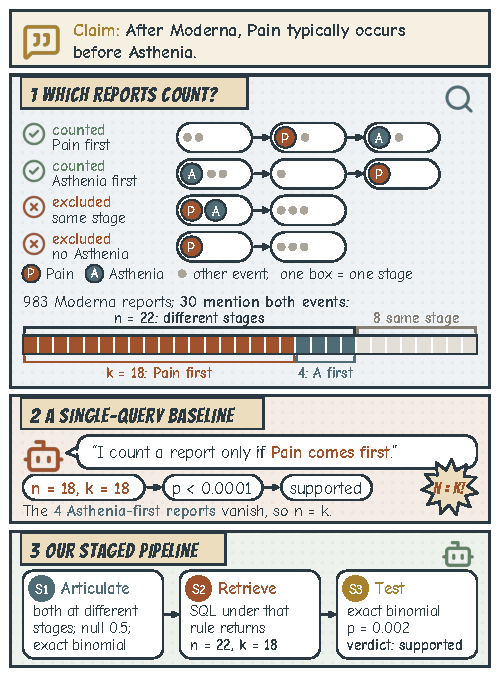
\includegraphics[width=\columnwidth]{Figures/worked_example.pdf}
\caption{One test claim end to end, with real counts. (1) Four Moderna
reports, one per case; the bar splits the 30 reports that mention both
events into the denominator $n$ and the numerator $k$. (2) A single-query
baseline and (3) our staged pipeline, both run with the same open model
(\S\ref{sec:baselines}, \S\ref{sec:method}).}
\label{fig:example}
\end{figure}

\begin{figure*}[t]
\centering
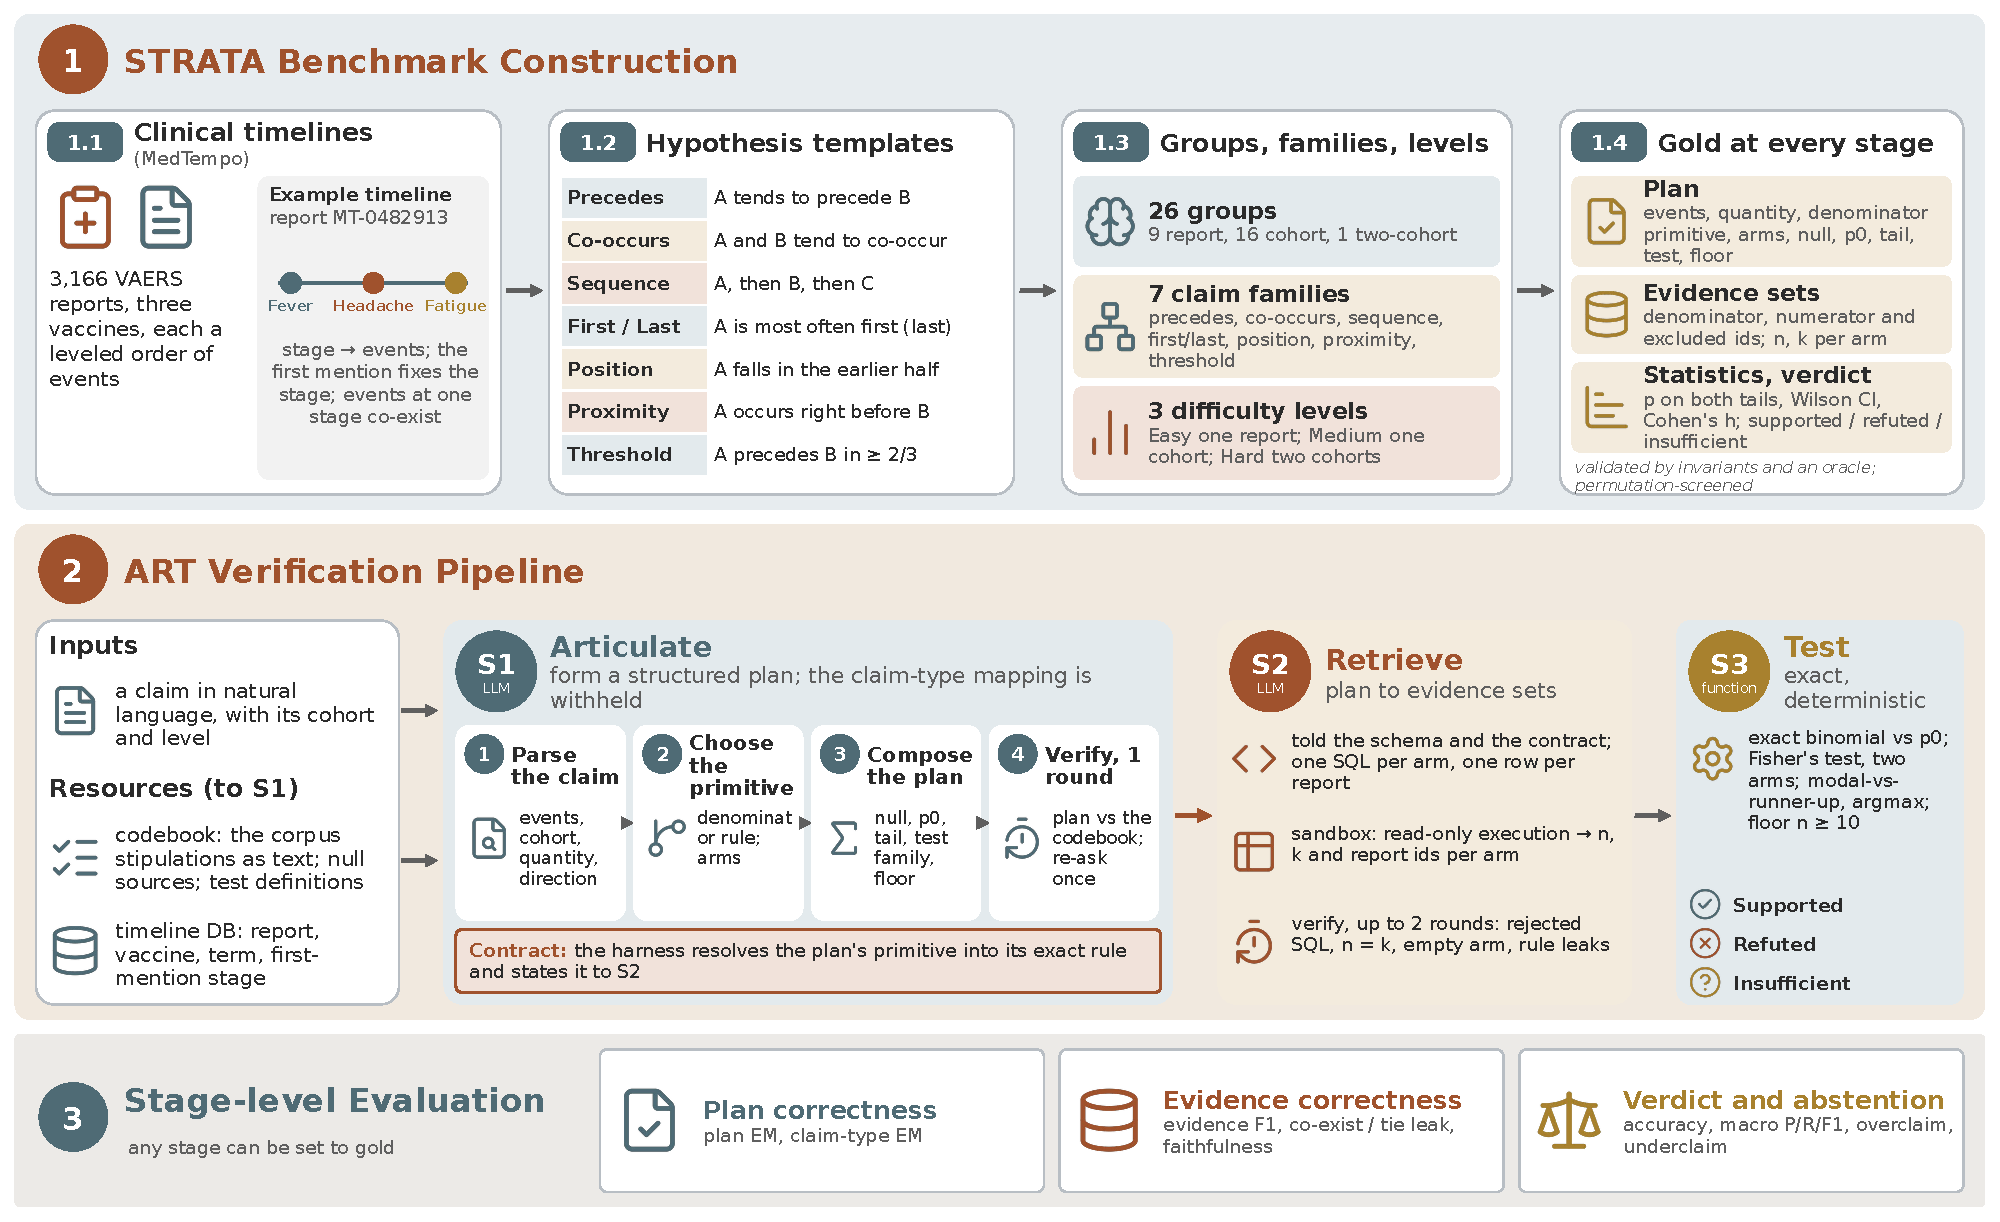
\includegraphics[width=\textwidth]{Figures/overview_slide.pdf}
\caption{Overview. Top: \sys{} benchmark construction, from the clinical
timelines (1.1) through the hypothesis templates (1.2) and the groups,
families and difficulty levels (1.3) to the gold computed at every stage
(1.4). Bottom: the \art{} verification pipeline, articulate (S1), retrieve
(S2) and test (S3), with the contract between S1 and S2 and the
verify-and-repair loops; beneath each stage, the measure that scores its
output against the gold (3).}
\label{fig:overview}
\end{figure*}

\section{Related Work}
\label{sec:related}

Work on language models and statistical hypotheses ranges from choosing a
test to running a whole analysis. StatQA \cite{zhu2024statqa} asks which test
applies, StatFormBench \cite{wang2026statformbench} asks for the formulation
of a test family, and StatABench \cite{zhu2026statabench} scores the final
answer of an analysis run with fixed tool functions. P-Bench and Fisher-R1
\cite{miao2026fisher} are closest to our setting: an agent receives a
hypothesis with its null stated, a CSV of the relevant data and a glossary,
writes R to compute a $p$-value, and is scored on the decision and the
$p$-value. Agentic systems go further and plan the analysis themselves. LATCH
\cite{gim2026latch} runs LLM-chosen analyses through deterministic R pipelines
on EHR data with the method given, VERITAS \cite{veritas2026} is a multi-agent
co-scientist with a deterministic evidence classifier for image-derived
cohorts, and DiscoveryBench and BLADE
\cite{majumder2025discoverybench,gu2024blade} evaluate open-ended discovery
agents against rubrics. Across this line of work the data are either handed
over as the relevant subset or left entirely to the agent, the hypotheses
concern variables in a table, and only the final answer or a rubric is
scored. None asks the system to decide which records a statistic is computed
over, and none releases gold for that decision or for the plan and the test
around it.

Temporal reasoning with language models has mostly been evaluated on single
texts. Benchmarks ask about the order, duration or frequency of events in a
passage or a synthetic event graph \cite{wang2024tram,fatemi2025testoftime};
clinical temporal relation extraction labels the order of events within one
narrative \cite{sun2013i2b2,bethard2016clinicaltempeval}; and TIMER
\cite{timer2025} and CRAFT \cite{craft2026} extract and refine clinical
timelines with language models. Clinical question answering over databases
likewise asks for one answer per question, with an abstention option in
EHRSQL \cite{lee2022ehrsql} and with a code-writing agent and error-driven
retries in EHRAgent \cite{shi2024ehragent}, and open text-to-SQL models such
as OmniSQL \cite{li2025omnisql} are built for the same setting. In all of these the answer is a fact about one text,
one timeline or one query. A temporal hypothesis is a claim about a
population of timelines, and verifying it adds the decisions this paper
scores: which timelines can witness the order at all, what chance looks like
when events crowd the early stages, and which exact test decides. \sys{}
starts where extraction ends, using the MedTempo timelines released with
CRAFT as its data source, and adapts EHRSQL, EHRAgent and DiscoveryBench as
baselines (\S\ref{sec:baselines}); Table~\ref{tab:related-concise}
(Appendix~\ref{app:positioning}) compares the closest work point by point.

\iffalse  % prose positioning table kept in source only (user 2026-10-21); Table~\ref{tab:related-concise} is the live one
\begin{table*}[t]
\centering
\scriptsize
\setlength{\tabcolsep}{3pt}
\renewcommand{\arraystretch}{1.15}
\begin{tabularx}{\textwidth}{@{}p{2.55cm} Y Y Y Y Y Y@{}}
\toprule
Work & Formulates the null? & Statistic computed by & Event-order claims & Clinical & Gold at intermediate stages & Dataset-in interface \\
\midrule
P-Bench / Fisher-R1 \cite{miao2026fisher} & no; $H_0$ given, test chosen but unscored & model-written R in a sandbox & no (survival only) & partly & no; final $p$ and decision & no; 425 fixed tasks \\
LATCH \cite{gim2026latch} & no; hypothesis and method both given & deterministic R pipelines & no (cross-sectional) & yes (NHANES) & partial; cohort $n$, CI vs.\ the paper & yes; schema summary \\
StatFormBench \cite{wang2026statformbench} & family label only & nothing computed & no & textbook & formulation only & no \\
StatABench \cite{zhu2026statabench} & test selection, no null & fixed tool functions & no & no & final answer & no \\
StatQA \cite{zhu2024statqa} & applicability only & nothing computed & no & no & final answer & no \\
DiscoveryBench / BLADE \cite{majumder2025discoverybench,gu2024blade} & open-ended hypothesis & agent code & no & no & rubric / expert & no \\
EHRAgent / EHRSQL \cite{shi2024ehragent,lee2022ehrsql} & no (QA / SQL) & agent code / SQL & no & yes (EHR) & answer / execution & schema \\
VERITAS \cite{veritas2026} & plans the analysis & own code + deterministic classifier & no & yes (imaging) & verdict vs.\ reference & data + description \\
\midrule
\textbf{This work} & \textbf{yes}: null recipe (kind, $p_0$ or how to compute it, reference population), denominator, test family + rule & \textbf{deterministic harness} runs the stated rule; exact tests & \textbf{yes}: precedes, co-occur, sequence, first/last, position, proximity, threshold & \textbf{yes}: VAERS timelines & \textbf{every stage}: plan, evidence set, counts, $p$, verdict & stated codebook + dataset card \\
\bottomrule
\end{tabularx}
\caption{Positioning against the closest benchmarks and systems. ``Gold at
intermediate stages'' is what makes per-stage attribution possible;
``event-order claims'' means hypotheses about the order or timing of events
within a record.}
\label{tab:related}
\end{table*}
\fi

\section{The \sys{} Benchmark}
\label{sec:dataset}

\subsection{Task definition}
\label{sec:task}

\sys{} gives each decision in the chain of \S\ref{sec:intro} its own gold, and
the timelines are its reference: a label is the decision the stipulated
procedure reaches on them. A record pairs a
temporal hypothesis, stated in natural language in one of four registers,
with the timelines: for every report, its vaccine and the stage at which
each event term is first mentioned. The hypothesis is about a \emph{cohort}
(the reports of one vaccine), a \emph{contrast} of two cohorts, or one named
\emph{report}. The system never sees report text. It must verify the
hypothesis by a statistical test over the timelines and return
\emph{supported}, \emph{refuted} or \emph{insufficient}. A claim is
supported when its own one-sided tail is significant at $\alpha = 0.05$ and
refuted when the opposite tail is. Otherwise it is insufficient, sub-typed
as \emph{not-locatable} (no report qualifies), \emph{sparse} (fewer than the
minimum count qualify) or \emph{underpowered} (enough qualify but neither
tail is significant; two thirds of these test claims have power below 0.8
at Cohen's $h = 0.5$ \cite{cohen1988}). Under a claim's null a decisive label
has probability at most 0.10, and 0.048 on average on the test set.

For a cohort-tier claim the gold is computed in three released steps: (1) a
\emph{plan}, giving the events, the quantity compared, the \emph{denominator
primitive} (which reports count), the number of arms, the null, the tail and
the test family; (2) the \emph{evidence}, the identifiers of the reports in
each arm's denominator and numerator; and (3) the exact test with its minimum
count. A report-tier claim is one deterministic reading of a report's timeline
and carries no test. Figure~\ref{fig:example} follows one test claim through
these steps.

Several readings of a claim depend on stipulations about the corpus, not
on the sentence: whether a report with both events at one stage counts for
``precedes'', or whether a tie for ``first'' leaves the denominator. The
benchmark ships these stipulations as the codebook (\S\ref{sec:frames}) and
withholds only the \emph{mapping} from wording to rule and test, which a
system is scored on composing.

\subsection{Benchmark construction}
\label{sec:construction}
\label{sec:corpus}

We use the clinical timelines of MedTempo~\cite{craft2026}: 3{,}166 VAERS
adverse-event reports for three COVID-19 vaccines (1{,}164 Janssen, 1{,}019
Pfizer, 983 Moderna; 1{,}660 event terms; 7.2 events and 3.4 stages per
report on average), each represented as a \emph{leveled order}, a chain of
stages in which each stage holds the MedDRA-coded events reported at that
point. A term's \emph{first} mention fixes its stage, and events at one stage
\emph{co-exist}, with no order between them. Systems receive the timelines, not
the narratives, so an error is one of verification; reading the narratives
is the task CRAFT studies.

\label{sec:space}\label{sec:realization}
Hypotheses come from 26 template groups in seven claim families:
\emph{precedes}, \emph{co-occurs}, \emph{sequence} of three events,
\emph{first/last} among candidates, and, to diversify the null,
\emph{position} (an event in the earlier half of a timeline),
\emph{proximity} (two events at consecutive stages) and \emph{threshold} (a
rate of at least a stated bar). They span three difficulty levels:
\emph{Easy} claims read one report's timeline (9 groups), \emph{Medium}
claims test a rate within one cohort (16 groups), and \emph{Hard} claims
compare two cohorts (1 group). Figure~\ref{fig:overview} shows one template
per family, and Table~\ref{tab:catalogue} (Appendix~\ref{app:catalogue})
lists every group. Each group is rendered in four registers
(\textsc{Original}, \textsc{Research}, \textsc{Media}, \textsc{Clinical}) by
mechanical slot-filling, with no model-written text. Every decisive core is
posed both ways, as a \emph{supported} claim and its \emph{refuted} mirror
over identical evidence, so a system that supports both directions of one
fact is caught. Each cohort group ships equal thirds of
supported, refuted and insufficient claims, so its fixed wording cannot
predict the label, and a seeded draw caps it at 600 instances while keeping
mirror pairs together. \emph{Not-locatable} claims are
minted from real cohort vocabulary whose joint count is zero, so the claim
looks answerable and only querying the timelines reveals the empty
denominator.

\label{sec:gold}
Gold labels are computed mechanically from the timelines. The denominator
rule of each family is the substance of the task. \emph{Precedes} counts
only reports with both events at distinct stages; \emph{co-occurs} counts
every report with both, because co-existence is what it asks about; and
\emph{first/last} drops reports in which candidates tie. The catalogue gives
every rule. Five kinds of null appear: the symmetric $0.5$ for order claims,
the named cell against its strongest competitor for argmax claims, equality
of two rates for contrasts, a bar read off the wording for threshold claims,
and a rate derived from the data for position and proximity claims. Order
and bar claims use a one-sided exact binomial. Data-derived nulls use a
one-sided binomial at the mean of the per-report chance rates. It is
conservative whenever its rejection cutoff lies at least one count beyond
the expected count \cite{hoeffding1956}, which holds in both tails for every
such test claim; under the exact Poisson-binomial its decisive rate is 0.050,
and the exact test changes 1 of the 180 labels. Argmax claims use an exact binomial of the named cell against its
strongest observed competitor. In the claim's direction this is an
intersection--union test against every competitor, with size at most
$\alpha$ \cite{berger1982}, because the binomial $p$-value grows with the
competitor's count. Contrasts use Fisher's exact test
\cite{fisher1935design}. The only gate is a minimum denominator of 10 per
arm. Each instance releases both one-sided $p$-values, the Wilson interval
\cite{wilson1927} and Cohen's $h$ \cite{cohen1988}, oriented to the claim as
asserted.

\label{sec:screens}
Before shipping, every group cleared a permutation null matched to its claim
shape \cite{good2005permutation}, under which decisive labels fall to about
$\alpha$ of the cores (5.1--5.3\% for position claims, against 14--15\% with a
naive null of 0.5). Six families of mechanical invariants are
checked over all 56{,}138 instances the templates enumerate, before the
per-group cap that leaves the released pool of 8{,}763. A
deterministic oracle that parses each template back into the reference SQL
reproduces every gold label, so the labels follow from the stated rules.

\label{sec:release}\label{sec:stats}
The release (Table~\ref{tab:stats}) contains a 1{,}500-claim test set, a
seeded verdict-balanced draw of up to 90 claims per cohort group,
fact-disjoint from a 200-instance development set, a 180-claim single-report
case study, and the full enumerated pool of 8{,}763 instances with its
generator. Inputs and gold are in separate files, every report identifier is
a keyed pseudonym of its VAERS identifier, and a \texttt{fact\_id} keys every
split. The full release, with the code, follows acceptance.

\begin{table}[t]
\centering
\small
\setlength{\tabcolsep}{4pt}
\begin{tabular}{@{}lr@{}}
\toprule
Test set (Medium / Hard claims) & 1{,}500 (1{,}418 / 82) \\
Single-report case study (Easy claims) & 180 \\
Development set & 200 \\
Groups / families / difficulty levels & 26 / 7 / 3 \\
Registers per claim & 4 \\
Enumerated pool: instances (records) & 8{,}763 (35{,}052) \\
\quad supported / refuted / insufficient & 3{,}521 / 3{,}521 / 1{,}721 \\
\quad underpowered / sparse / not-locatable & 605 / 498 / 618 \\
Test denominator $n$, median (IQR) & 21 (14--41) \\
$|$Cohen's $h|$ on decisive claims, median & 0.65 \\
\bottomrule
\end{tabular}
\caption{The release. Per-group sizes are in the claim catalogue
(Appendix~\ref{app:catalogue}).}
\label{tab:stats}
\end{table}

\section{Method}
\label{sec:framework}
\label{sec:method}
\label{sec:contracts}
\label{sec:verify}

\art{} turns the three gold steps of \S\ref{sec:task} into three stages,
so that each decision is an output that can be scored
(Figure~\ref{fig:overview}). It \emph{articulates} the claim as a plan
naming its temporal conditioning rule, null and exact test,
\emph{retrieves} the report sets the plan conditions on, and \emph{tests}
them with a deterministic exact test, so the verdict is a statistical
decision rather than a model judgment. Each stage has an output contract and
can be scored against its gold or filled with gold. The two model stages
also have a bounded verify-and-repair loop that reads only the contract, the
codebook and the data, never the gold. Unless stated otherwise, \art{}
includes these loops.

\subsection{S1: Articulate}
\label{sec:frames}

From the record (text, level, cohort) the model composes a plan:
\texttt{events}, \texttt{quantity}, \texttt{denominator} (a named primitive:
\emph{ordered\_pair}, \emph{both\_present}, \emph{all\_present\_unique\_first},
\emph{consecutive\_pair}, \emph{present\_offmid}, \emph{presence\_split},
\emph{single\_report}, \ldots), \texttt{arms}, \texttt{null\_kind} with $p_0$
or a reference population, \texttt{tail}, \texttt{test\_family} and a rule for
the floor. The prompt states the codebook by situation (``a report with two
events tied for earliest has no answer and is excluded''; ``order words are
distance-blind; only wording that says the two are adjacent conditions on
consecutive stages''). It adds a computed dataset card, the null sources and
the test definitions. It withholds the mapping from wording to claim type,
so the model composes the plan instead of looking it up. The prompt is
zero-shot, since a worked plan would be a row of that mapping. The harness
derives the claim type from the plan by reverse lookup over its fields; a
plan that names no known shape is \emph{underdetermined} and scored as
insufficient. The plan is then checked for consistency with the codebook (a
quantity against its denominator, a null kind against its situation, a
stated bar against the wording, a valid test family) and re-asked once with
the violations named.

\subsection{S2: Retrieve}

For each arm the model writes one SQL statement over the timeline database
(two tables, two views) that returns \emph{one row per report} with four
flags: in the denominator, in the numerator, excluded, and an optional cell
label for argmax claims. The plan reaches this stage as a \emph{contract}:
the harness resolves the plan's claim type and writes that type's
conditioning rule and arm plan into the prompt, so the model receives the
rule for the one primitive the plan names. The ablation without the contract
hands over the plan's JSON with the full codebook as \emph{prose} instead
(\S\ref{sec:modular}). The harness executes the
statement in a read-only sandbox and aggregates the rows into $(n, k)$ per arm
with the identifier sets, so the evidence is auditable against the gold
sets. A statement the database rejects, an arm whose denominator equals its
numerator, an empty arm beside a full one, and rows that violate the plan's
primitive (co-existing reports in an order denominator, ties in a first/last
denominator, non-consecutive pairs in an immediate denominator) trigger a
re-ask, up to two rounds. The checks are defined against the plan, so the
loop is part of the staged design: the baselines run as their protocols
define them, and with only the plan-free checks a single query gains
0.04--0.06 (the 2024 pair and gemma4) where \art{} gains 0.05--0.14
(\S\ref{sec:modular}).

\subsection{S3: Test}

A deterministic function runs the plan's test on the counts
(Table~\ref{tab:catalogue}): the exact binomial against the plan's $p_0$ (for
a data-derived null, $p_0$ is the mean chance over the retrieved
denominator), Fisher's test for two arms, and modal-versus-runner-up for
argmax claims. It applies the floor and returns the verdict with both tails.
Nothing is inferred at this stage, so it needs no verification.

\section{Experiments}
\label{sec:experiments}

\subsection{Research questions}
\label{sec:rqs}

The experiments ask whether systems make the decisions of
\S\ref{sec:task} correctly and whether their verdicts show it. Each
question is answered on the test set, with the same five models in every
model slot.

\begin{itemize}
\item \textbf{RQ1.} How well do current language models verify these
temporal hypotheses end to end, as a single query or as an agent, and where
do they fail?
\item \textbf{RQ2.} What does the staged pipeline add over a single query,
and which stages and claim families account for the remaining errors?
\item \textbf{RQ3.} Do correct verdicts rest on correct evidence, and how
often do systems decide claims the data cannot decide, or abstain on claims
it can?
\end{itemize}

\subsection{Baselines}
\label{sec:baselines}

Three published systems are adapted to the benchmark, all over the same
database. \emph{EHRSQL} \cite{lee2022ehrsql} follows the single-query
text-to-SQL protocol: one prompt per claim asks for one query over our schema
that marks each report as in the denominator, the numerator or neither, and
the harness runs the query and the exact test. \emph{EHRSQL-C} adds the
codebook to the prompt, so it differs from \art{} only in having no plan, no
contract and no repair. \emph{EHRAgent} \cite{shi2024ehragent} runs as
released, writing and executing its own code with up to twelve error-driven
retries and four demonstrations, and running its own test; it receives the
schema, the exact-test functions and the floors but not the codebook, since
its knowledge stage writes the plan itself. \emph{DiscoveryBench}'s reference
agent \cite{majumder2025discoverybench} runs as released on the same tables
exported as CSV, with the codebook as its domain knowledge, an instruction to
end on a verdict line and up to 25 steps. At one to two minutes per claim,
it runs on a stratified 204-claim subsample (Appendix~\ref{app:subsample}).
The two agents run as released and show how autonomous analysis fares on the
task; they are not matched controls.

\emph{Stage baselines} replace one stage of \art{} with an established method
for that step and set the other stages to gold. For Articulate, a plain prompt
gives the model the dataset description, the codebook and the plan schema,
without \art{}'s explanations, field rules or verify round, with and without
zero-shot chain-of-thought \cite{kojima2022zeroshot}. For Retrieve, OmniSQL
\cite{li2025omnisql}, fine-tuned from the same base as our 2024 SQL model,
writes the SQL from the gold plan. For Test, the StatQA protocol
\cite{zhu2024statqa} gives the model the gold counts and the test definitions
and asks for the test and the verdict. The matching \art{} rows fill the same
stage with \art{}'s own component; the Articulate row, whose plan is compiled
to SQL and tested exactly, is a deterministic-compilation pipeline.

\subsection{Evaluation metrics}
\label{sec:metrics}

The verdict is scored as a three-class prediction, by accuracy and by
precision, recall and F1 macro-averaged over \emph{supported},
\emph{refuted} and \emph{insufficient}. These numbers cannot show whether a
right verdict rests on the right evidence, so the stage gold is used to
score the steps behind it. \emph{Plan EM} is exact match on the plan's
fields. Four evidence measures follow (Figure~\ref{fig:families}).
\emph{Evidence F1} is the F1 between the reports a system placed in an arm's
denominator and the gold set, averaged over arms. \emph{Faithfulness} is the
share of correct verdicts whose denominator is exactly the gold set in every
arm. \emph{Overclaim} is the share of gold-\emph{insufficient} claims
given a decisive verdict, and \emph{underclaim} is the share of decisive
claims answered \emph{insufficient}.

\subsection{Experimental settings}
\label{sec:setup}

Every result in Table~\ref{tab:main} is on the 1{,}500-claim test set (\S\ref{sec:release}), run
once in the \textsc{Original} register after every prompt was frozen on the
development set. A review copy with the development set, its gold at every
stage, the timeline database, \art{}'s outputs on the development set and a
scorer is at \url{https://anonymous.4open.science/r/STRATA-WWW2027/}. Every system is run with each of five models in every
model slot: the 2024 open pair Qwen2.5-32B-Instruct (planning) and
Qwen2.5-Coder-32B (SQL) \cite{qwen2025qwen25}; the 2026 open models
qwen3.8-27B \cite{qwen2026qwen38} and gemma4-31B \cite{gemma2026gemma4}, one
model for both stages, thinking off; and the frontier models Claude Opus~5.5
\cite{anthropic2026opus55} and GPT-5.6 \cite{openai2026gpt56}. Open models run fully resident on one RTX A5000 with an 8k
context, frontier models over their APIs. Verdict
accuracies carry 95\% bootstrap intervals \cite{efron1993bootstrap} over
instances (1{,}000 resamples). Per-claim cost
and latency are in Appendix~\ref{app:cost}. All experiments, development
runs included, took about 355 GPU-hours and \$243 in API fees.

\section{Results}
\label{sec:results}

% Main table: split layout (one column per score under each model, user 2026-10-22) is live; the
% previous one-cell-per-model layout is kept below. Set \splitmaintablefalse to switch back.
\newif\ifsplitmaintable \splitmaintabletrue
\ifsplitmaintable
\begin{table*}[t]
\centering
\footnotesize
\setlength{\tabcolsep}{2.4pt}
\renewcommand{\arraystretch}{1.12}
\begin{tabular}{@{}lrrrr@{\hspace{6pt}}rrrr@{\hspace{6pt}}rrrr@{\hspace{6pt}}rrrr@{\hspace{6pt}}rrrr@{}}
\toprule
test set, 1{,}500 cohort claims & \multicolumn{4}{c}{\textbf{Qwen2.5-32B pair}} & \multicolumn{4}{c}{\textbf{qwen3.8-27B}} & \multicolumn{4}{c}{\textbf{gemma4-31B}} & \multicolumn{4}{c}{\textbf{Opus 5.5}} & \multicolumn{4}{c}{\textbf{GPT-5.6}} \\
\cmidrule(lr){2-5}\cmidrule(lr){6-9}\cmidrule(lr){10-13}\cmidrule(lr){14-17}\cmidrule(lr){18-21}
 & Acc & P & R & F1 & Acc & P & R & F1 & Acc & P & R & F1 & Acc & P & R & F1 & Acc & P & R & F1 \\
\midrule
\multicolumn{21}{@{}l}{\textit{adapted baselines}} \\
EHRSQL & .529 & .555 & .528 & .518 & .587 & .605 & .587 & .582 & .635 & .647 & .634 & .629 & .878 & .882 & .878 & .878 & .876 & .877 & .876 & .876 \\
EHRSQL-C & .575 & .604 & .574 & .570 & .748 & .764 & .747 & .748 & .859 & .885 & .858 & .861 & 1.000 & 1.000 & 1.000 & 1.000 & .984 & .984 & .984 & .984 \\
EHRAgent & .605 & .694 & .606 & .600 & .839 & .863 & .839 & .843 & \multicolumn{4}{c}{---} & \multicolumn{4}{c}{---} & .792 & .808 & .792 & .794 \\
DiscoveryBench$^\dagger$ & \multicolumn{4}{c}{---} & .647 & .812 & .647 & .711 & .706 & .784 & .706 & .729 & \multicolumn{4}{c}{---} & \multicolumn{4}{c}{---} \\
\midrule
\multicolumn{21}{@{}l}{\textit{adapted stage baselines (other stages at gold)}} \\
Articulate: \art{} & .953 & .985 & .953 & .969 & .917 & .942 & .917 & .928 & .992 & .992 & .992 & .992 & .993 & .993 & .993 & .993 & .993 & .993 & .993 & .993 \\
\quad plain prompt & .867 & .920 & .867 & .892 & .859 & .913 & .859 & .882 & .923 & .936 & .922 & .927 & \multicolumn{4}{c}{---} & \multicolumn{4}{c}{---} \\
\quad plain prompt + chain-of-thought & .923 & .957 & .922 & .938 & .863 & .925 & .862 & .891 & .912 & .920 & .912 & .913 & \multicolumn{4}{c}{---} & \multicolumn{4}{c}{---} \\
Retrieve: \art{} & .836 & .879 & .835 & .840 & .944 & .945 & .944 & .944 & .989 & .990 & .989 & .989 & \multicolumn{4}{c}{$\geq$.999 on all four} & \multicolumn{4}{c}{$\geq$.999 on all four} \\
\quad OmniSQL-32B$^\ddagger$ & .772 & .814 & .771 & .775 & \multicolumn{4}{c}{---} & \multicolumn{4}{c}{---} & \multicolumn{4}{c}{---} & \multicolumn{4}{c}{---} \\
Test: \art{} (exact test) & 1.000 & 1.000 & 1.000 & 1.000 & 1.000 & 1.000 & 1.000 & 1.000 & 1.000 & 1.000 & 1.000 & 1.000 & 1.000 & 1.000 & 1.000 & 1.000 & 1.000 & 1.000 & 1.000 & 1.000 \\
\quad StatQA & .611 & .706 & .609 & .575 & .619 & .784 & .617 & .539 & .777 & .816 & .776 & .776 & .999 & .999 & .999 & .999 & .999 & .999 & .999 & .999 \\
\midrule
\multicolumn{21}{@{}l}{\textit{ablations of \art{}}} \\
\quad $-$ verify-and-repair & .761 & .845 & .760 & .777 & .735 & .815 & .734 & .744 & .844 & .886 & .843 & .848 & .999 & .999 & .999 & .999 & .999 & .999 & .999 & .999 \\
\quad $-$ exact test (model verdict) & .512 & .651 & .510 & .482 & .568 & .612 & .566 & .503 & .770 & .809 & .769 & .769 & \multicolumn{4}{c}{---} & \multicolumn{4}{c}{---} \\
\quad $-$ contract (plan as prose) & .663 & .704 & .663 & .671 & .841 & .870 & .841 & .851 & .947 & .948 & .947 & .947 & \multicolumn{4}{c}{---} & \multicolumn{4}{c}{---} \\
\midrule
\multicolumn{21}{@{}l}{\textit{ours}} \\
\textbf{\art{}} & \textbf{.810} & \textbf{.876} & \textbf{.809} & \textbf{.827} & \textbf{.872} & \textbf{.895} & \textbf{.872} & \textbf{.882} & \textbf{.981} & \textbf{.982} & \textbf{.981} & \textbf{.981} & \textbf{.993} & \textbf{.993} & \textbf{.993} & \textbf{.993} & \textbf{.983} & \textbf{.983} & \textbf{.983} & \textbf{.983} \\
\bottomrule
\end{tabular}
\caption{Main results on the test set. Under each model: verdict accuracy
(Acc) and macro precision, recall and F1 (P, R, F1) over the three verdict
classes, leading zeros dropped; only the model changes across column groups. Intervals on accuracy are $\pm 0.02$ (0.6--0.9) and
$\pm 0.01$ (above 0.98). Every baseline is adapted to \sys{}: it reads the
same timeline database and returns the three-way verdict, and its name
identifies the protocol or released system, not its original setting
(\S\ref{sec:baselines}). $^\ddagger$Fine-tuned from Qwen2.5-Coder-32B, so
listed under the 2024 pair. $^\dagger$Run on a stratified 204-claim subsample
(Appendix~\ref{app:subsample}), with the two 2026 open models. A dash marks a run not made.}
\label{tab:main}
\end{table*}
\else
\begin{table*}[t]
\centering
\scriptsize
\setlength{\tabcolsep}{3.5pt}
\renewcommand{\arraystretch}{1.12}
\begin{tabular}{@{}lrrrrr@{}}
\toprule
test set, 1{,}500 cohort claims & \textbf{Qwen2.5-32B pair} & \textbf{qwen3.8-27B} & \textbf{gemma4-31B} & \textbf{Opus 5.5} & \textbf{GPT-5.6} \\
 & \multicolumn{5}{c}{\textit{Verdict accuracy \,(macro precision / recall / F1)}} \\
\midrule
\multicolumn{6}{@{}l}{\textit{adapted baselines}} \\
EHRSQL & 0.529\,{\scriptsize(0.555/0.528/0.518)} & 0.587\,{\scriptsize(0.605/0.587/0.582)} & 0.635\,{\scriptsize(0.647/0.634/0.629)} & 0.878\,{\scriptsize(0.882/0.878/0.878)} & 0.876\,{\scriptsize(0.877/0.876/0.876)} \\
EHRSQL-C & 0.575\,{\scriptsize(0.604/0.574/0.570)} & 0.748\,{\scriptsize(0.764/0.747/0.748)} & 0.859\,{\scriptsize(0.885/0.858/0.861)} & 1.000\,{\scriptsize(1.000/1.000/1.000)} & 0.984\,{\scriptsize(0.984/0.984/0.984)} \\
EHRAgent & 0.605\,{\scriptsize(0.694/0.606/0.600)} & 0.839\,{\scriptsize(0.863/0.839/0.843)} & --- & --- & 0.792\,{\scriptsize(0.808/0.792/0.794)} \\
DiscoveryBench$^\dagger$ & --- & 0.647\,{\scriptsize(0.812/0.647/0.711)} & 0.706\,{\scriptsize(0.784/0.706/0.729)} & --- & --- \\
\midrule
\multicolumn{6}{@{}l}{\textit{adapted stage baselines (other stages at gold)}} \\
Articulate: \art{} & 0.953\,{\scriptsize(0.985/0.953/0.969)} & 0.917\,{\scriptsize(0.942/0.917/0.928)} & 0.992\,{\scriptsize(0.992/0.992/0.992)} & 0.993\,{\scriptsize(0.993/0.993/0.993)} & 0.993\,{\scriptsize(0.993/0.993/0.993)} \\
\quad plain prompt & 0.867\,{\scriptsize(0.920/0.867/0.892)} & 0.859\,{\scriptsize(0.913/0.859/0.882)} & 0.923\,{\scriptsize(0.936/0.922/0.927)} & --- & --- \\
\quad plain prompt + chain-of-thought & 0.923\,{\scriptsize(0.957/0.922/0.938)} & 0.863\,{\scriptsize(0.925/0.862/0.891)} & 0.912\,{\scriptsize(0.920/0.912/0.913)} & --- & --- \\
Retrieve: \art{} & 0.836\,{\scriptsize(0.879/0.835/0.840)} & 0.944\,{\scriptsize(0.945/0.944/0.944)} & 0.989\,{\scriptsize(0.990/0.989/0.989)} & $\geq$0.999 & $\geq$0.999 \\
\quad OmniSQL-32B$^\ddagger$ & 0.772\,{\scriptsize(0.814/0.771/0.775)} & --- & --- & --- & --- \\
Test: \art{} (exact test) & 1.000 & 1.000 & 1.000 & 1.000 & 1.000 \\
\quad StatQA & 0.611\,{\scriptsize(0.706/0.609/0.575)} & 0.619\,{\scriptsize(0.784/0.617/0.539)} & 0.777\,{\scriptsize(0.816/0.776/0.776)} & 0.999\,{\scriptsize(0.999/0.999/0.999)} & 0.999\,{\scriptsize(0.999/0.999/0.999)} \\
\midrule
\multicolumn{6}{@{}l}{\textit{ablations of \art{}}} \\
\quad $-$ verify-and-repair & 0.761\,{\scriptsize(0.845/0.760/0.777)} & 0.735\,{\scriptsize(0.815/0.734/0.744)} & 0.844\,{\scriptsize(0.886/0.843/0.848)} & 0.999\,{\scriptsize(0.999/0.999/0.999)} & 0.999\,{\scriptsize(0.999/0.999/0.999)} \\
\quad $-$ exact test (model verdict) & 0.512\,{\scriptsize(0.651/0.510/0.482)} & 0.568\,{\scriptsize(0.612/0.566/0.503)} & 0.770\,{\scriptsize(0.809/0.769/0.769)} & --- & --- \\
\quad $-$ contract (plan as prose) & 0.663\,{\scriptsize(0.704/0.663/0.671)} & 0.841\,{\scriptsize(0.870/0.841/0.851)} & 0.947\,{\scriptsize(0.948/0.947/0.947)} & --- & --- \\
\midrule
\multicolumn{6}{@{}l}{\textit{ours}} \\
\textbf{\art{}} & \textbf{0.810\,{\scriptsize(0.876/0.809/0.827)}} & \textbf{0.872\,{\scriptsize(0.895/0.872/0.882)}} & \textbf{0.981\,{\scriptsize(0.982/0.981/0.981)}} & \textbf{0.993\,{\scriptsize(0.993/0.993/0.993)}} & \textbf{0.983\,{\scriptsize(0.983/0.983/0.983)}} \\
\bottomrule
\end{tabular}
\caption{Main results on the test set: verdict accuracy, then macro
precision / recall / F1 over the three verdict classes; only the model
changes across columns. Intervals on accuracy are $\pm 0.02$ (0.6--0.9) and
$\pm 0.01$ (above 0.98). Every baseline is adapted to \sys{}: it reads the
same timeline database and returns the three-way verdict, and its name
identifies the protocol or released system, not its original setting
(\S\ref{sec:baselines}). $^\ddagger$Fine-tuned from Qwen2.5-Coder-32B, so
listed under the 2024 pair. $^\dagger$Run on a stratified 204-claim subsample
(Appendix~\ref{app:subsample}), with the two 2026 open models. A dash marks a run not made.}
\label{tab:main}
\end{table*}
\fi


\iffalse  % evidence table kept in source; Figure~\ref{fig:families} carries these metrics (user 2026-10-20)
\begin{table*}[t]
\centering
\small
\setlength{\tabcolsep}{5pt}
\begin{tabular}{llrrrrr}
\toprule
metric & system & Qwen2.5-32B pair & qwen3.8-27B & gemma4-31B & Opus 5.5 & GPT-5.6 \\
\midrule
evidence F1 & B & 0.643 & 0.751 & 0.836 & 1.000 & 1.000 \\
 & D$'$ + verifier & 0.789 & 0.914 & 0.975 & 0.998 & 0.993 \\
faithfulness & B & 0.405 & 0.693 & 0.859 & 1.000 & 1.000 \\
 & D$'$ + verifier & 0.859 & 0.972 & 0.945 & 0.998 & 0.999 \\
overclaim & B & 0.234 & 0.141 & 0.036 & 0.000 & 0.000 \\
 & D$'$ + verifier & 0.033 & 0.047 & 0.010 & 0.004 & 0.020 \\
underclaim & B & 0.388 & 0.224 & 0.182 & 0.000 & 0.001 \\
 & D$'$ + verifier & 0.223 & 0.068 & 0.023 & 0.009 & 0.011 \\
\bottomrule
\end{tabular}
\caption{Evidence and abstention on the test set for the Straight-to-SQL control
(B) and our pipeline. Denominator F1 is over the report sets each arm
retrieved; faithfulness is $P(\text{denominator exact} \mid \text{verdict
right})$; overclaim is the share of gold-\emph{insufficient} claims
given a decisive verdict; underclaim the share of decisive claims
answered \emph{insufficient}.}
\label{tab:evidence}
\end{table*}
\fi

Table~\ref{tab:main} reports every system, the stage baselines and the
ablations on the same 1{,}500 claims.

\subsection{RQ1: end-to-end verification}
\label{sec:main}

End to end, accuracy depends on whether the system is told the codebook.
Without it, a single query verifies 0.53--0.88 of the claims across the five
models (EHRSQL in Table~\ref{tab:main}); with it, the same query reaches
0.58--1.00 (EHRSQL-C). The gain grows with the model's ability to apply the
text: 0.05 for the 2024 pair, 0.16 for qwen3.8, 0.22 for gemma4 and
0.11--0.12 for the frontier models, which then verify 0.98--1.00 of the
claims with every denominator but one exact. Frontier models, then, fail
only for lack of the corpus rules. The 2024 pair cannot apply them: given
the codebook, it stops admitting most co-existing reports into order
denominators but starts writing queries that define the eligible set as the
supporting set ($n = k$, 325 claims), and gains almost nothing.

Without the codebook, every error is a wrong rule about which reports can
witness a temporal claim, and Appendix~\ref{app:attribution} names the rule
for each claim. The frontier models' errors fall on four rules: first/last
denominators that admit reports missing one of the candidates (102--150
claims, first/last accuracy 0.66--0.74); adjacency counted across
co-existing events (35--63 claims, proximity 0.79--0.90); position claims
over reports that have no earlier half (up to 31); and order and
co-occurrence denominators that admit reports with only one of the events.
The open models make the same errors in larger numbers and add the one the
codebook states first, co-existing reports in order denominators (281--325
claims). In each case the query runs and counts the wrong reports.

Agents that write and run their own analysis do no better. Without the
codebook, EHRAgent's retries help the models that also fail the single
query, by 0.08 for the 2024 pair and 0.25 for qwen3.8, but cost GPT-5.6 0.08
(0.792 against 0.876). Free to choose, GPT-5.6 keeps ties in first/last
denominators, applies multiple-comparison corrections and counts
co-occurrence over reports with either term, each a defensible convention
that is not this corpus's. Given the codebook, DiscoveryBench's agent scores
below the single query with the same model on the same 204 claims: 0.65 and
0.71 against 0.76 and 0.88 for qwen3.8 and gemma4
(Appendix~\ref{app:subsample}), where every other system scores within its
own test-set interval. A likely cause is that an agent writes its own
denominator and test, so it has more places to depart from the codebook, and
nothing checks the departure.

\begin{figure*}[t]
\centering
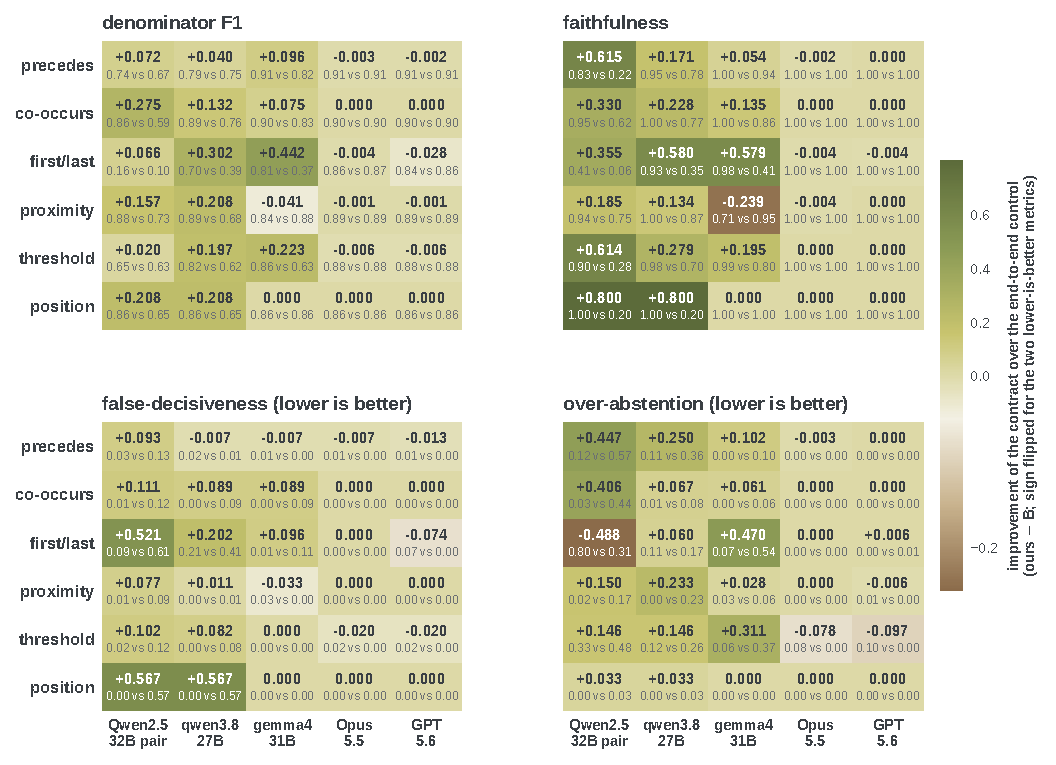
\includegraphics[width=\textwidth]{Figures/families.pdf}
\caption{The four evidence measures of \art{} on the test set, by claim
family and model, drawn as error rates so that 0 is perfect in every panel:
the share of wrongly counted reports ($1-$evidence F1), of right verdicts
resting on the wrong evidence ($1-$faithfulness), of undecidable claims
decided (overclaim) and of decidable claims abstained on (underclaim). The
colour scale is square-root, so small errors remain visible.}
\label{fig:families}
\end{figure*}

\subsection{RQ2: the staged pipeline and where errors remain}
\label{sec:families}

Under \art{}, every open model gains 0.12 to 0.24 in verdict accuracy over
EHRSQL-C, and gemma4-31B comes within 0.02 of the frontier with no marginal API fees.
The gain comes from the contract and the repair loop together
(\S\ref{sec:modular}). The contract takes the interpretation of the
codebook out of the SQL the model writes, and \S\ref{sec:evidence} shows the
same gain in the evidence. The frontier models score the same under \art{}
as end to end. The repair loop costs them a little, because its checks flag
a few correct $n = k$ statements and \art{} then abstains instead of
guessing. For them \art{} adds an auditable record of plan, report sets and
test, which a single query does not produce.

\iffalse  % family table kept in source; Figure~\ref{fig:groups} (ours by group) and Figure~\ref{fig:families} (evidence vs B) carry it (user 2026-10-20)
\begin{table*}[t]
\centering
\small
\setlength{\tabcolsep}{5pt}
\begin{tabular}{lrrrrrr}
\toprule
family (D$'$ + verifier / B) & $n$ & Qwen2.5-32B pair & qwen3.8-27B & gemma4-31B & Opus 5.5 & GPT-5.6 \\
\midrule
precedes (P-V1--P-V4, P-M2) & 455 & 0.802 / 0.571 & 0.811 / 0.741 & 0.998 / 0.932 & 0.996 / 1.000 & 0.989 / 1.000 \\
co-occurs (C-V1--C-V3) & 270 & 0.974 / 0.570 & 0.963 / 0.878 & 1.000 / 0.930 & 1.000 / 1.000 & 1.000 / 0.915 \\
first/last (F-V1--F-V3) & 262 & 0.435 / 0.332 & 0.798 / 0.584 & 0.950 / 0.565 & 1.000 / 1.000 & 0.973 / 0.996 \\
proximity (Y-V1--Y-V3) & 271 & 0.985 / 0.753 & 1.000 / 0.801 & 0.970 / 0.963 & 1.000 / 1.000 & 0.996 / 1.000 \\
threshold (H-V1, H-V5) & 152 & 0.763 / 0.605 & 0.901 / 0.743 & 0.961 / 0.750 & 0.941 / 1.000 & 0.914 / 1.000 \\
position (T-V1) & 90 & 1.000 / 0.722 & 0.689 / 0.722 & 1.000 / 1.000 & 1.000 / 1.000 & 1.000 / 1.000 \\
\bottomrule
\end{tabular}
\caption{Verdict accuracy by claim family on the test set, our pipeline with
the verifier against the Straight-to-SQL control, same model. The sequence family
has no cohort-tier group in the test set (its two cohort groups have four
cores each in the corpus) and appears in the report-tier case study only.}
\label{tab:families}
\end{table*}
\fi

Accuracy under \art{} varies by claim family, and each model fails on
different families (Figure~\ref{fig:families-radar},
Appendix~\ref{app:families-radar}). The 2024 pair loses on two families
whose rule it cannot carry out: first/last, an argmax over three candidates
with ties dropped from the denominator, and threshold, where one group
states its bar in the text. The 2026 open models clear first/last. qwen3.8
misses position, whose null is a data-derived rate, and the precedes variant
that compares two antecedents (P-V2); gemma4 misses only proximity and
threshold. Threshold is the one family where the frontier models also drop.
Their planner-alone rows drop by the same amount, so the loss is in
composing the bar into the plan, not in retrieval.

\begin{figure}[t]
\centering
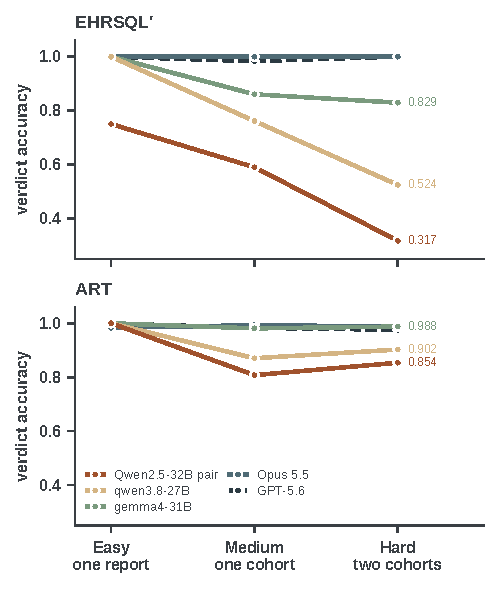
\includegraphics[width=\columnwidth]{Figures/tiers.pdf}
\caption{Verdict accuracy on one claim shape, \emph{A precedes B}, at the
three difficulty levels: E, read off one report (P-R1, 20 claims); M, tested
in one cohort (P-V1, 95); H, compared across two cohorts (P-M2, 82). One
panel per model: \art{} against EHRSQL-C, which shares its model, codebook,
database and exact test but has no plan, contract or repair. Bands are 95\%
Wilson intervals over claims.}
\label{fig:tiers}
\end{figure}

The three levels contain different families, so their pooled accuracies
would mix difficulty with family. Figure~\ref{fig:tiers} holds the claim
shape fixed instead and compares \art{} with EHRSQL-C. Under \art{} every model
verifies the single-report and one-cohort claims, and the open models lose
0.15 (pair), 0.10 (qwen3.8) and 0.01 (gemma4) when a second cohort adds a
second denominator and a two-sample test. EHRSQL-C loses 0.68, 0.48 and 0.17
over the same steps, the pair already 0.38 at the one-cohort step, while the
frontier models stay at or near 1.0 in both systems. The contract cuts the
cost of the harder level by a factor of 4.7 for the 2024 pair, 4.9 for
qwen3.8 and 14 for gemma4.

On the 180 single-report claims, every system given the codebook scores
0.98--1.00 with a 2026 or frontier model, and the 2024 pair reaches 1.000
only under \art{} (0.750 as a single query). Rewording the test claims in the
three other registers costs the open models up to 0.13 under \art{}, and for
the 2026 models the planner alone loses the same amount, so paraphrase is
paid at planning (Figure~\ref{fig:registers}, Appendix~\ref{app:registers}).

\subsection{RQ3: evidence and abstention}
\label{sec:evidence}
\label{sec:insufficient}

Every prediction records the reports it counted, so each verdict can be
checked against the gold sets. End to end, the verdict overstates what a
system computed, which is the verdict--evidence gap. EHRSQL-C rests 40\% (pair), 69\% (qwen3.8) and 86\%
(gemma4) of its right verdicts on the exact denominator, so only 0.23 of
the pair's 0.575 accuracy is right for the right reason. Panel 2 of
Figure~\ref{fig:example} shows one such case from qwen3.8: the query admits
only the reports that support the claim, so $n = k$ and the verdict is
\emph{supported} whatever the data say. Under \art{} the same shares are
86\%, 97\% and 94\%, a larger gain than in accuracy and largest for the
weakest model; the frontier models are exact on all but a handful of claims
in both systems. Over the whole executed trace (both sets in every arm, test,
null kind and verdict), \art{} is right on 0.62, 0.81 and 0.92 of claims for
the open models against 0.21, 0.51 and 0.73 for EHRSQL-C. The frontier
models score 0.95--0.96 against 0.98--1.00 for EHRSQL-C, which is given the
gold test, and miss mostly on H-V5. The agents cannot be checked this way, because EHRAgent
and DiscoveryBench's agent return a verdict from their own code without the
reports behind it.



Figure~\ref{fig:families} breaks \art{}'s evidence down by claim family.
Almost every cell is at or near zero error for gemma4 and the frontier
models, and for most families of qwen3.8; overclaim stays at a few percent
everywhere. Each remaining dark cell has a cause the plan exposes. The 2024
pair retrieves the wrong set on first/last and abstains on four claims in
five, qwen3.8 overclaims on first/last, and the frontier models underclaim
on threshold, the H-V5 slip discussed below. One failure does not show in
the verdicts: gemma4 is right on 0.97 of proximity claims, but a fifth of
those right verdicts rest on a denominator that admits non-adjacent pairs.
EHRSQL-C is weaker on the same families, with faithfulness of 0.06--0.41 on
first/last for every open model.

\begin{figure}[t]
\centering
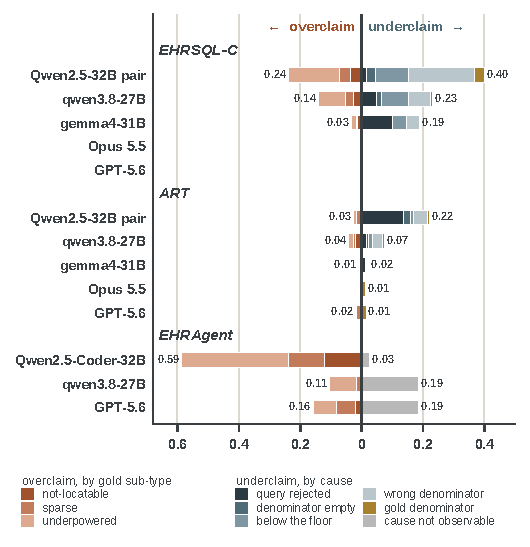
\includegraphics[width=\columnwidth]{Figures/insufficient.pdf}
\caption{The \emph{insufficient} class on the test set, one row per system
and model. Left: overclaim, by gold sub-type. Right: underclaim, by cause;
grey where the cause is not observable. Numbers are row totals.}
\label{fig:insufficient}
\end{figure}

Figure~\ref{fig:insufficient} separates deciding what the data cannot decide
from abstaining on what they can. Overclaim is the share of the
505 gold-\emph{insufficient} claims (176 \emph{not-locatable}, 157
\emph{sparse}, 172 \emph{underpowered}) given a decisive verdict. Underclaim
is the share of the 995 decisive claims answered \emph{insufficient}, split by
what the prediction shows, which is also the sub-type the system claimed: an
empty denominator claims \emph{not-locatable}, one below the floor
\emph{sparse}, a testable one \emph{underpowered}. EHRAgent returns a bare
verdict, so its causes cannot be observed.

Overclaim comes mostly from the agents and the single-query baselines. EHRAgent
with the Coder decides more than half of the undecidable claims and nearly
all \emph{underpowered} ones, because it runs its own test. EHRSQL-C
overclaims mostly on \emph{underpowered} claims, where a wrong denominator
moves the tail, and fills \emph{not-locatable} denominators with reports
that do not qualify. \art{} overclaims on a few percent at most, because the
exact test, not the model, abstains, and its abstentions name the right
sub-type on 0.87--1.00 of claims against 0.79--1.00 for EHRSQL-C.

Underclaim is concentrated in the open models. The single query with the
2024 pair abstains on nearly four decisive claims in ten, mostly on a wrong
denominator or one below the floor. The stronger EHRAgent models trade
overclaim for underclaim, not for correct verdicts. Under \art{}, the pair's
abstentions are mostly queries that still fail after two repairs. The
frontier models' few abstentions all fall in one group, H-V5, where the plan
reads a stated bar as an argmax claim and runs the wrong test on the right
counts.

\subsection{Ablations}
\label{sec:modular}

The ablations in Table~\ref{tab:main} remove one part of \art{} at a
time: the verify-and-repair loops; the exact test, replaced by the model's
own verdict from \art{}'s counts; and the contract, with the plan handed to
S2 as prose with the codebook. Removing both the plan and the contract
leaves EHRSQL-C.


\iffalse  % modular table merged into Table~\ref{tab:main} (user 2026-10-20); kept in source
\begin{table*}[t]
\centering
\small
\setlength{\tabcolsep}{5pt}
\begin{tabular}{lrrrrr}
\toprule
stages filled by the model (the others at gold) & Qwen2.5-32B pair & qwen3.8-27B & gemma4-31B & Opus 5.5 & GPT-5.6 \\
\midrule
S1: plan, with the verifier (2 repair rounds) & 0.953 & 0.917 & 0.992 & 0.993 & 0.993 \\
S2: retrieval, with the verifier (2 repair rounds) & 0.836 & 0.944 & 0.989 & $\geq$0.999 & $\geq$0.999 \\
LLM verdict from the gold counts (S1, S2 at gold; replaces S3) & 0.611 & 0.619 & 0.777 & 0.999 & 0.999 \\
S1 + S2 with the verifier + LLM verdict from the model's own counts & 0.512 & 0.568 & 0.770 & --- & --- \\
\midrule
S1 + S2 + S3 (ours, no verifier) & 0.761 & 0.735 & 0.844 & 0.999 & 0.999 \\
\textbf{S1 + S2 + S3 + verifier (ours)} & \textbf{0.810} & \textbf{0.872} & \textbf{0.981} & 0.993 & 0.983 \\
\bottomrule
\end{tabular}
\caption{Modular analysis on the test set. S1, S2 and S3 are the pipeline's
plan, retrieval and exact-test stages; S3 is deterministic, so the rows
that replace it with an LLM verdict from the counts are ablations of the
design, not stages of it. Each row names what the model fills, with every
other stage at gold; with all stages at gold the harness reproduces the
labels exactly (1.000). S2 is run under the same resolved contract the full
pipeline uses, so the difference between the S2 row and the S1$+$S2$+$S3 rows
is the cost of the model's own plan. The frontier S2 cells are not run
separately: with their own plans both models retrieved every denominator
exactly (evidence F1 1.000 in Figure~\ref{fig:families}), which bounds the
gold-plan row from below.}
\label{tab:modular}
\end{table*}
\fi

\iffalse  % stage-ceilings figure dropped (user 2026-10-20): it repeats rows of Table~\ref{tab:main}
\begin{figure*}[t]
\centering
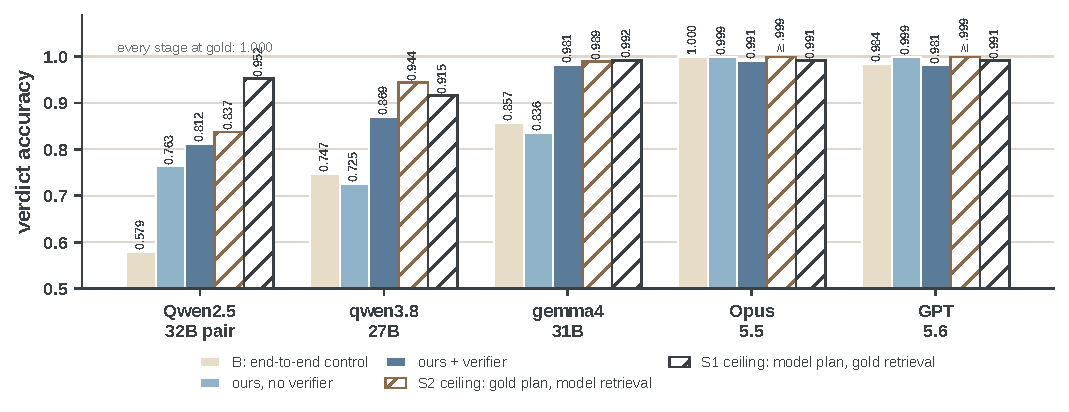
\includegraphics[width=\textwidth]{Figures/modular.pdf}
\caption{The stage-ceiling block of Table~\ref{tab:main} as bars: for each model the end-to-end
control, our pipeline without and with the verifier, and the two stage
ceilings as outlined bars, the model's retrieval with the gold plan (S2) and
the model's plan with gold retrieval (S1); every stage at gold is the line at
1.000. The contract and the verifier carry the 2024 pair from 0.575 to within
0.03 of its retrieval ceiling and gemma4 from 0.859 to within 0.01 of both
ceilings; the frontier models are at the ceilings with or without the
contract.}
\label{fig:modular}
\end{figure*}
\fi

The stage rows in Table~\ref{tab:main} fill one stage with the model and
leave the others at gold, so each row measures the loss from that stage
alone. With the mapping withheld and the codebook given, every model
composes the right plan on at least nine claims in ten, and the gemma4
planner matches the frontier. A plain prompt with the same codebook and plan
schema but without \art{}'s explanations, field rules and verify round
scores 0.86--0.92 with or without zero-shot chain-of-thought, below
\art{}'s planner for every open model (0.92--0.99; exact McNemar on the
paired claims, $p < 0.001$). Retrieval is where the 2024 pair loses: its
Coder drops a sixth of the claims even with the gold plan, so the full
pipeline adds planner errors to a stage that already fails. The 2026 models
retrieve well with the gold plan, so their remaining loss is the plan, and
gemma4 under \art{} sits within 0.01 of both its stage rows. The open models
do not compute the test reliably. Under the StatQA protocol on the exact
counts they are wrong on a fifth to two fifths of claims, and replacing the
exact test with the model's verdict on \art{}'s own counts loses 0.2 to
0.3.

The stage rows cannot measure the hand-off between S1 and S2, because
Retrieve receives the gold plan already resolved. The \emph{$-$ contract}
row hands the same composed plan to S2 as prose with the codebook, so only
the resolution of the named primitive into its rule is removed. This costs the 2024 pair 0.15 of
verdict accuracy (0.810 to 0.663) and the 2026 models 0.03 (0.872 to 0.841
for qwen3.8, 0.981 to 0.947 for gemma4). Without the contract the pair is
barely above a single query with the same codebook and the same two repair
rounds (0.638), while the 2026 models keep most of \art{}'s gain over
EHRSQL-C (0.748 and 0.859). The weaker the model, the more of \art{}'s gain
the contract carries.
% The development-set version of this comparison (prose below verified EHRSQL-C; contract +~0.3)
% is kept in the repo only (appendix.tex, commented section app:dev).

\begin{figure}[t]
\centering
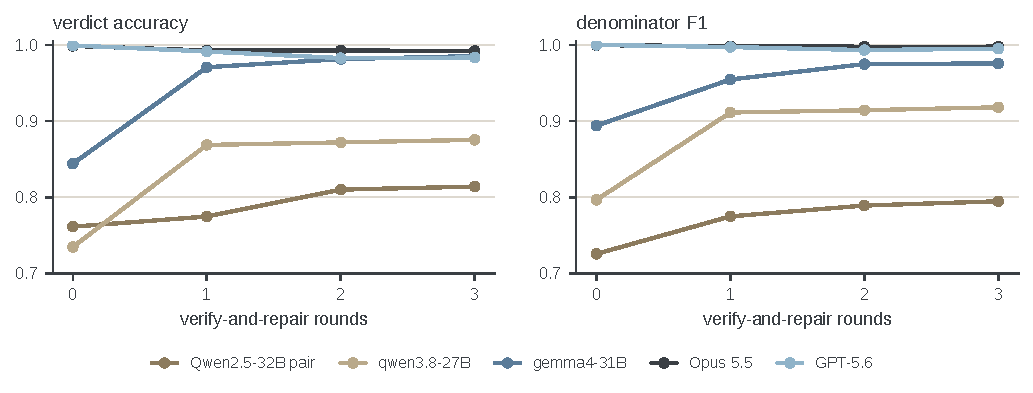
\includegraphics[width=\columnwidth]{Figures/rounds.pdf}
\caption{What each verify-and-repair round adds: the change in verdict
accuracy from the previous round, for rounds one to three, on the test set;
gains extend to the right, losses to the left.}
\label{fig:rounds}
\end{figure}

With zero to three verify-and-repair rounds (Figure~\ref{fig:rounds}), the
first round gives the 2026 open models about
$+0.13$ and later rounds a few thousandths, while each round costs the
frontier models a little; two rounds is the operating point for every open
model.

\iffalse  % repair-rounds table kept in source; Figure~\ref{fig:rounds} carries it (user 2026-10-20)
\begin{table}[t]
\centering
\small
\setlength{\tabcolsep}{4pt}
\begin{tabular}{lrrrrr}
\toprule
rounds & Qwen2.5 pair & qwen3.8 & gemma4 & Opus 5.5 & GPT-5.6 \\
\midrule
0 & 0.761 / 0.726 & 0.735 / 0.797 & 0.844 / 0.894 & 0.999 / 1.000 & 0.999 / 1.000 \\
1 & 0.775 / 0.775 & 0.869 / 0.911 & 0.971 / 0.955 & 0.993 / 0.998 & 0.991 / 0.997 \\
2 & 0.810 / 0.789 & 0.872 / 0.914 & 0.981 / 0.975 & 0.993 / 0.998 & 0.983 / 0.993 \\
3 & 0.814 / 0.795 & 0.875 / 0.918 & 0.985 / 0.976 & 0.992 / 0.998 & 0.983 / 0.995 \\
\bottomrule
\end{tabular}
\caption{Our pipeline with 0--3 verify-and-repair rounds on the test set:
verdict accuracy / evidence F1.}
\label{tab:rounds}
\end{table}
\fi

\iffalse  % registers table kept in source; Figure~\ref{fig:registers} carries it (user 2026-10-20)
\begin{table}[t]
\centering
\small
\begin{tabular}{lrrrr}
\toprule
development set, 32B pair & Original & Research & Media & Clinical \\
\midrule
planner alone (S2, S3 at gold), 1 round & 0.965 & 0.850 & 0.860 & 0.935 \\
D$'$ & 0.865 & 0.790 & 0.755 & 0.825 \\
D$'$ + verifier & 0.870 & 0.815 & 0.770 & 0.840 \\
B (Straight-to-SQL control) & 0.640 & 0.587 & 0.600 & 0.557 \\
\bottomrule
\end{tabular}
\caption{Verdict accuracy by register on the 200 development instances
(claim form).}
\label{tab:registers}
\end{table}
\fi

\section{Conclusion}
\label{sec:limitations}
\label{sec:conclusion}

\sys{} turns temporal hypothesis verification into a chain of scored
decisions: which reports can witness a claim, what the null is, which exact
test applies and what the evidence was. It exposes a verdict--evidence gap:
systems fail at the first of these, and the verdict does not show it. Frontier models verify the claims once the
codebook is stated. Open models need the plan as a contract; with it, a 31B
model on one GPU comes within 0.02 of the frontier with an auditable
denominator, while models asked to make the statistical call themselves err
even on exact counts. Benchmarks of this kind should publish their codebook
with their data and score the evidence with the answer.

The study has five limits. It uses one corpus, so porting the framework
means writing the codebook and primitives for another corpus. The claims are generated from
templates over raw MedDRA terms, so their wording varies only across the four
registers, and the oracle shows that labels follow from the stated rules, not
that free-form wording would carry them; clinician-written claims and
held-out templates are the next step. Decisive labels carry false positives
at up to $\alpha$ per direction by construction. In P-V2 and P-V4 a report can
qualify for both arms, which Fisher's test treats as independent; a
randomization test that keeps each shared report's two outcomes paired changes
2 of their 188 test labels and reverses none. And the patterns are regularities in
spontaneous reports, not causal findings.
